\section{\label{qleet-sec:abstract}Abstract}

Manipulating a target object using a fixed-base robot manipulator presents a complex problem that requires addressing multiple constraints, such as optimizing the manipulator joint cost, finding a collision-free trajectory, and modeling the object dynamics. Previous approaches have relied on contact-rich manipulation, where the object moves predictably while attached to the manipulator, thereby avoiding the need to model the object's dynamics, which does not generalize to multiple types of end-effectors. Further, collision avoidance for manipulators in existing approaches rely on context-specific neural network-based object representation, which need to be retrained for each specific arrangement and type of obstacles and robots.  
We first discuss a stochastic trajectory optimizer, Via-point Stochastic Trajectory Optimization and adapt it for context-agnostic path planning in the joint space for commonly-used robot manipulators, such as the Franka Panda and UR5e. Next, we propose a novel framework that disentangles the non-prehensile long-horizon manipulation problem into planning and control. The planning component uses the aforementioned context-agnostic Via-Point stochastic trajectory optimizer, generating a collision-free trajectory from the start to the goal position, consisting of multiple via-points. This simplifies the task of the reinforcement learning based control component, which only needs to move the object closer to the next via-point. We pair the high-level via-point planner with a low-level push controller based on Deep Reinforcement Learning, that is gripper-agnostic. A key contribution of our approach is that the planning module predicts the most optimal path for the control component given the scene context using a bi-level optimization scheme. Our experimental results demonstrate that the proposed framework can generalize to arbitrary scenes with multiple collision objects of different shapes and sizes. We evaluate the framework on a few complex scenes using a two-fingered gripper and show improvements over different related approaches.

\section{Introduction}

Object manipulation is an essential task for robots to perform that has many diverse downstream applications, for example in the service industry (manipulating kitchenware~\cite{kitchen_arm}), industrial setting (packaging~\cite{industrial_arm}) and household (tabletop rearrangement~\cite{agarwal2022approaches}). Broadly, object manipulation can be of two types - \textit{Prehensile}, which involves continuous contact-rich gripping of the object using the manipulator's end-effector(gripper or a hand-like structure), and \textit{Non-Prehensile}, which involves moving the object without grasping it. Prehensile actions are often used in manufacturing, packaging, and assembly processes where the robot needs to handle and manipulate objects of various shapes and sizes. On the other hand, non-prehensile actions are typically used when the object is too fragile or too large to be picked up by the robot's gripper. Instead, the robot uses other methods such as pushing, pulling, sliding, or rolling to move the object around. Non-prehensile manipulator actions are commonly used in applications such as warehouse automation, sorting, and material handling.

Path planning for manipulators involves finding a collision-free path for a robot arm or manipulator to follow as it moves from its current position to a desired position. Any trajectory sent to a manipulator to be followed must satisfy the dynamic and kinematic constraints of the robot, as well as the workspace bounds in which it operators. A few commonly-used approaches to path planning for manipulators include the following:

\begin{itemize}
    \item \textit{Sampling-based Methods:} These methods randomly sample the configuration space of the robot (i.e., the set of all possible positions and orientations) and attempt to find a collision-free path by connecting the samples together. Examples of sampling-based methods include Rapidly-exploring Random Trees(RRTs)\cite{RRT-og} and Probabilistic Roadmaps (PRMs)\cite{PRM}.
    \item \textit{Search-based Methods:} These methods search for a path through the configuration space using a search algorithm, such as A*\cite{A*} or Dijkstra's algorithm. Search-based methods can be combined with heuristics to reduce the search space and improve performance.
    \item \textit{Optimization-based Methods:} These methods formulate the path planning problem as an optimization problem, where the objective is to find the shortest path that satisfies certain constraints (e.g., collision avoidance). Optimization may be performed by gradient-based updates, or by sampling potential candidates from a distribution and updating the distribution itself after evaluating the cost over the candidates. 

\end{itemize}

In this chapter, we will explore optimization-based methods for path planning for manipulators. Sections \ref{sec:bg-gradient-manipulator} and \ref{sec:bg-sampling-manipulator} provide a background of standard gradient-based and sampling-based optimization approaches for robot manipulation, respectively. We adapt an improved version of stochastic trajectory optimization from Section \ref{sec:bg-sampling-manipulator} for our purpose and incorporate it into a bi-level push planner for manipulators. The contributions of this chapter is twofold:

\begin{itemize}
    \item Designing a fast, collision-aware high-level global path planner using stochastic trajectory optimization for manipulators
    \item Coupling this high-level planner with a low-level push controller to enable the manipulator to perform precise long-horizon non-prehensile actions, such as pushing an object on a table.
\end{itemize}

\section{High-level Global Planning for Manipulators}

In this section, we introduce the basics of high-level path planning algorithm, Via-Point Stochastic Trajectory Optimization(VP-STO)\cite{VPSTO}, and design a suitable joint-space cost function incorporating collision-avoidance. We show a few simulation results of our high-level global planner on the Universal Robots, UR5e robot arm and the Franka Emika Panda robot arm, both of whose kinematics have been discussed in Section \ref{sec:bg-manipulator-kinematics}.


\subsection{Via-Point Stochastic Trajectory Optimization(VP-STO)}

Via-Point Stochastic Trajectory Optimization(VP-STO)\cite{VPSTO} fits different candidate trajectories satisfying the start and goal constraints to perform stochastic optimization over a cost function. VPSTO computes $N$ via-points between the start and the goal by sampling them from a multivariate Gaussian distribution, and fits trajectories satisfying the kinematic constraints of the robot and the workspace passing through them. The cost corresponding to these trajectories are then evaluated, and the trajectories are ranked in their order of cost. Finally the parameters of the sampling distribution are updated using the Covariance-Matrix Adaptation Method (CMA-ES). The benefit of the CMA-ES approach over standard Cross-Entropy Methods(CEM) lies in the following factors:

\begin{itemize}
    \item \textit{Better handling of non-linearities}: CMA-ES is known for its ability to handle non-linear optimization problems, which are common in manipulator planning. CEM, on the other hand, tends to struggle with non-linearities, which can result in slower convergence and suboptimal solutions.
    \item \textit{Adaptive step size:} CMA-ES uses an adaptive step size to adjust the search direction and step size during optimization, which helps to avoid getting stuck in local optima. CEM, on the other hand, uses a fixed step size, which can lead to premature convergence and suboptimal solutions.
    \item \textit{Better exploration of search space:}  CMA-ES uses a probabilistic approach to explore the search space, which helps to avoid getting stuck in local optima and to find the global optimum. CEM, on the other hand, uses a deterministic approach, which can lead to poor exploration of the search space.
\end{itemize}

The overall optimization pipeline in VPSTO is denoted in Figure {\ref{fig:vpsto}}. The cost function can be represented as the following:

\begin{subequations}
\begin{align}
    min \int_{0}^{1}q''(s)^Tq''(s)ds \\
    \text{s.t} \qquad q(s_n) = q_n, \qquad n = 1,..,N \\
    q(0) = q_0, q'(0) = q_0', q(1) = q_T, q'(1) = q_T'
\end{align}
\end{subequations}



\begin{figure}[ht]
    \centering
    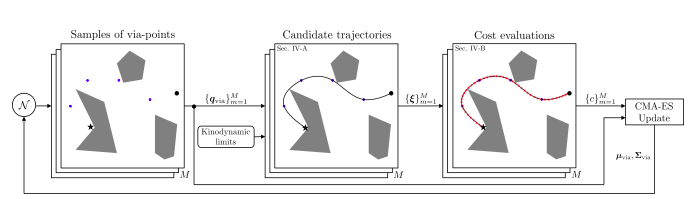
\includegraphics[scale=0.5]{figures/bl-manipulator/vpsto.png}
    \caption[The VPSTO pipeline]{The end-to-end pipeline for Via-Point Stochastic Trajectory Optimization(VP-STO). Source: \cite{VPSTO}}.
    \label{fig:vpsto}
\end{figure}


Here $s_n$ denotes the scaled via point timings $s_n = t_n/T$, which are uniformly distributed between $(0,1)$. $q(s)$ is a weighted sum of basis functions. $T$ is the total movement duration. Now, given the via-points $q_{via}$ and the boundary conditions $q_0$, $v_0$, $q_T$, $v_T$, the computation of the explicit continuous trajectory only depends on $T$. VPSTO approximates $T$ by solving for the minimum positive duration such that the resulting velocity and acceleration limits are satisfied over a discrete set of evaluation points, uniformly distributed in the continuous time space. 

For each evaluation point $s_k$, there exists a closed-form solution $T_k$ such that the motion happens through $q_0$, $q_T$, $q_{via}$, and the robot arm reach either the velocity limit or the acceleration limit at time $t = s_k$. VPSTO then picks the most conservative duration among the $K$ solutions for $T: T(q_{via}) = max(T_k)$, in order to make sure that the velocity and acceleration constraints are satisfied at all evaluation points. Once $T$ is known, $q(s)$ is found using the equations for $q_0$, $q_T$, $q_{via}$, $v_0$, and $v_T$. 

VPSTO optimizes the trajectory by minimizing a cost function that captures the tradeoff between smoothness, efficiency, and safety. Based on the design of the cost function that VPSTO minimizes, we can adapt it for a wide variety of applications. In this dissertation, we adapt the VPSTO algorithm for manipulator pushing tasks on a tabletop and pair it with a low-level push controller in Section \ref{sec:bi-level-method}.

\subsection{Collision Detection}

Collision detection for a robot manipulator needs to be performed on two fronts - self-collision, which involves collisions among the links of the robot itself, and environment collision, which includes collisions between the robot links and objects in the environment. Note that the contact between the robot's end-effector and the target object to be moved on the table is not considered as a collision. We have already discussed standard distance-based collision avoidance for manipulators in Section \ref{sec:distance-based-collision}. Let us now analyze the drawbacks of these existing approaches. 

As discussed in Section \ref{sec:distance-based-collision}, one way of checking for collisions is to sample points uniformly along the robot body and compute pairwise distances among them(for self-collision) and with other objects in the environment. If the computed distance exceeds the threshold separation determined by the geometries of the robot body and the objects, the point is collision-free. The difficulty with this approach arises due to its reliance on the knowledge of the exact geometries of the robot and the other objects. This makes it hard to generalize this approach across a range of objects of different shapes and sizes on the table, as well as to robots with different dynamics. Learning implicit representations of objects also runs into the same generalizability issue, and thus the necessity of a standardized approach capable of detecting collisions agnostic to object and robot geometries becomes evident. 

\subsubsection{PyBullet Mesh Overlap:}
In this chapter, we will adopt a different approach called 
\textit{Mesh Overlap}, that attempts to solve this problem of collision avoidance in a simulator setting. The simulator of our concern is PyBullet, which is a physics simulation engine that can be used to simulate robots and other complex systems in 3D. To use PyBullet to load 3D robots into a simulation scene, one can follow this  general sequence of steps:

\begin{enumerate}
    \item \textit{Define the robot model:} Start by defining the geometry, mass, and other properties of each link and joint in the robot model. This can be done using the URDF (Unified Robot Description Format) file format.
    \item \textit{Load the robot model:} Once we have defined the robot model, we can load it into PyBullet using the loadURDF function. This function takes as input the path to the URDF file and returns a unique identifier for the robot in the simulation.
    \item \textit{Visualize the robot:}\label{point:vis_robot} we can visualize the robot in PyBullet using the render function. This function generates a 3D mesh of the robot model and displays it in a window.
    \item \textit{Simulate the robot:} We can simulate the robot's behavior by applying forces and torques to its joints using the \verb_`setJointMotorControl2'_ function. This function allows we to specify the desired position, velocity, or torque for each joint in the robot model.
    \item \textit{Collect data:} During the simulation, we can collect data on the robot's position, velocity, and other properties using the \verb_`getBasePositionAndOrientation'_ and \verb_`getJointState'_ functions. This data can be used for analysis and control purposes.
\end{enumerate}

As discussed in point \ref{point:vis_robot}, the simulator contains the robot model as a set of geometric meshes. Similarly for objects in the environment, the simulator loads geometric meshes into the scene. An overlap between two object meshes indicates collision between them. We can, thus, detect collisions using PyBullet's inbuilt collision detection feature based on the overlap between the meshes of the robot and the obstacles, or between the meshes of robot links. In fact, PyBullet is equipped with the feature to detect collision by detecting mesh overlap and penetration depth between meshes through the function \verb_{getCollisionFn}_. An example of mesh overlap and subsequent collision detection in PyBullet is depicted in Figure \ref{fig:collisions-pybullet}.

\begin{figure}[ht]
    \centering
    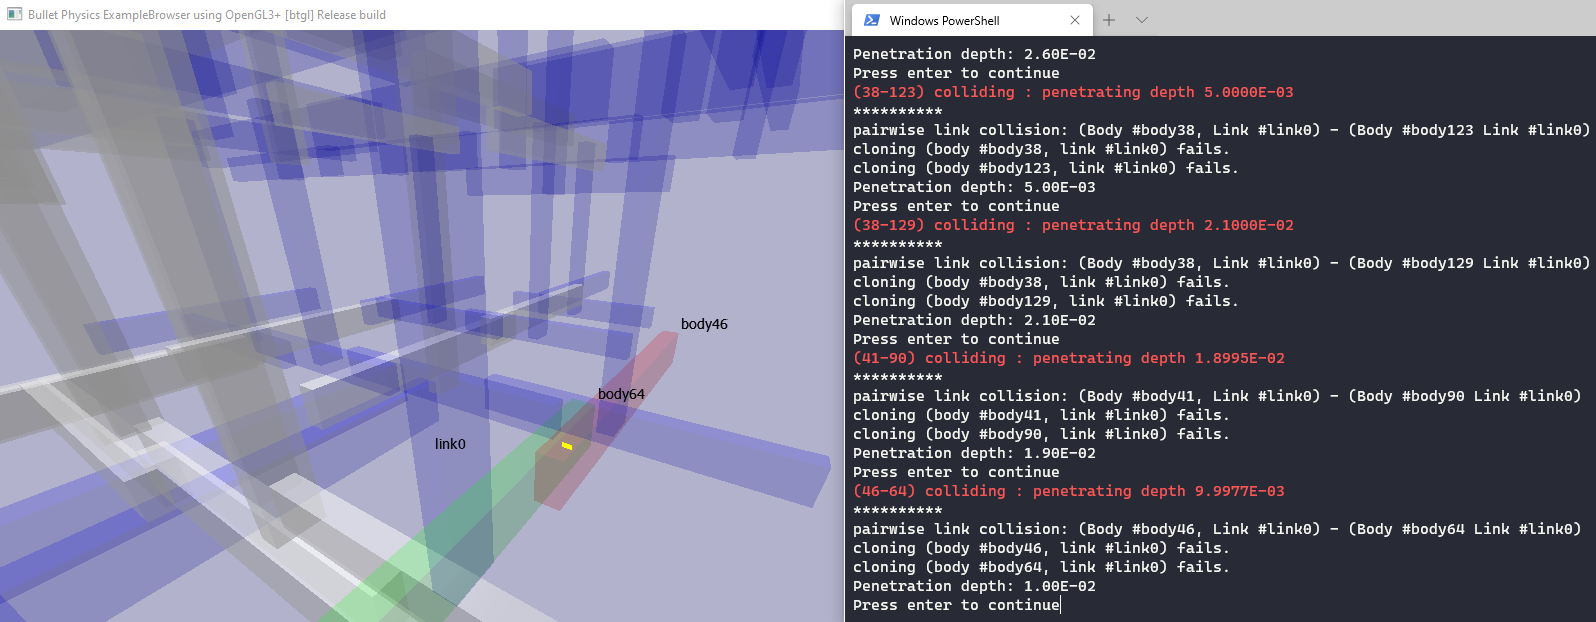
\includegraphics[scale=0.3]{figures/bl-manipulator/assembly_collision.png}
    \caption[Collision detection through Mesh Overlap]{Collision Detection through Mesh Overlaps in the PyBullet simulator. Source:  \scriptsize{\url{https://github.com/yijiangh/pybullet_planning_tutorials}}}
    \label{fig:collisions-pybullet}
\end{figure}

To explain PyBullet's inbuilt collision-detection through code, let us analyze the standard use of the \verb_getCollisionFn_ as follows:

\begin{verbatim}
    collision_fn = get_collision_fn(robot, ik_joints, obstacles, 
    self_collisions=True, disabled_collisions=self_collision_links)
    print (collision_fn(joint_poses, diagnosis = True))
\end{verbatim}

We send the robot model, list of movable joints, list of obstacle models to the \verb_getCollisionFn_, along with a few Boolean flags. \verb_selfCollisions_ indicates whether to detect self-collisions among the robot link meshes, \verb_disabledCollisionFn_ relaxes the collision detection between mesh pairs that are not be counted as a collision, for example, between the end-effector and the target object being moved. \verb_getCollisionFn_ returns a Boolean flag for a given snapshot of joint poses, indicating whether it has been able to detect a collision or not. The \verb_diagnosis_ flag indicates whether we want to visualize the detected collision in the PyBullet GUI or not.

\subsection{Joint-Space Path Planning}\label{sec:joint-cost}

The design of the cost function for VPSTO determines its application to the task at hand. For non-planar end-effector motion, such as grasping and pick-and-place operations, we perform global path-planning in the joint angle space. Recall from Section \ref{sec:bg-manipulator-kinematics} that the Franka Emika Panda robot has 7 movable joints, while the UR5e robot has 6 movable joints. To represent the joint angle movements and perform path-planning in the joint space, therefore, we would need to plan in 7-D for the Franka Panda manipulator and in 6-D for the UR5e manipulator. Joint-space planning allows us to also introduce joint limits as constraints into the optimization problem based on the robot dynamics. Note that we are allowed to design discontinuous non-differentiable cost functions since VPSTO never computes the gradient of the cost function, but relies on stochastic optimization. We design a cost function for VPSTO as a sum of the following terms:

\begin{enumerate}
    \item \textbf{Cost Limits}: This is defined as the frequency of violation of joint limits while executing a joint-space trajectory. 
    \item \textbf{Cost curvature}: Curvature cost aims to shorten the arc-length (refer to Section \ref{sec:traj_eval_metrics} for arc-length definition) of the joint-space trajectory to ensure short trajectories. 
    \item \textbf{Joint Cost}: Joint cost is defined as the norm of the difference in joint angles over successive timestamps. In essence, joint cost captures the effort expended by the robot to perform some task by changing its joint angles. 
    \item \textbf{Cost Collision}: This is a discrete cost, consisting of a very high cost value $C$ if a collision is detected, or 0 otherwise. 
    \begin{equation}
        \text{Collision Cost} = \begin{cases} 
      C & \text{if collision = True} \\
      0 & \text{otherwise} 
   \end{cases}
    \end{equation}
    
\end{enumerate}

\subsection{End-effector Space Planning}

For planar motion of the manipulator's end-effector, such as pushing an object along a table, we can discard the high-dimensional joint space path planning in favor of a simpler Cartesian-space motion of the end-effector. Thus the path planning for the end-effector can be performed in the Cartesian end-effector space, which would be 2-D in case of planar tabletop motion. The end-effector can be thought of as a circular holonomic robot in 2-D of diameter equivalent to the separation between the fingers of the gripper plus the finger widths. This approximation makes it possible to use standard holonomic robot path-planning algorithms, as well as stochastic optimizers like VPSTO to plan the end-effector trajectory. An example of a 2-D end-effector space trajectory for a manipulator is shown in Figure \ref{fig:end-eff-traj}.

\begin{figure}[ht]
    \centering
    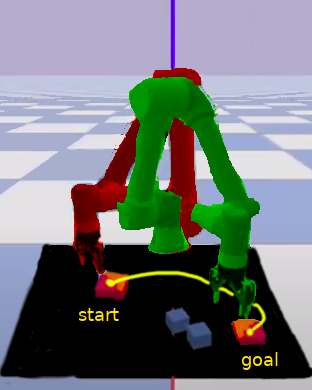
\includegraphics[scale=0.5]{figures/bl-manipulator/end_eff_traj.png}
    \caption[End-Effector trajectory in 2-D]{End-effector trajectory in 2-D for planar push motion on a tabletop. Here the red shaded manipulator denotes its start pose, and the green shaded manipulator denotes its final pose. The blue cubes indicate obstacles (collision objects) on the table. The end-effector motion happens along the plane of the black table, as the object moves from the start to the goal position. The yellow line denotes the trajectory of the centre of the object being pushed.}
    \label{fig:end-eff-traj}
\end{figure}

\subsection{Simulation Results}

We test the VPSTO-based global joint-space path planner using the cost function defined in Section \ref{sec:joint-cost} in PyBullet for a few scenarios involving one or two obstacles of varied sizes. The results of a few test simulations can be found at: \url{https://www.dropbox.com/scl/fo/t1dy47cgz2rvmedj9a87o/h?dl=0&rlkey=ou4losxv0i9lawc2wffnk60vl}. Figure \ref{fig:joint_traj_ur5} shows an example trajectory from our simulator runs for the Universal Robots UR5e robot arm. 

\begin{figure}[ht]
    \centering
    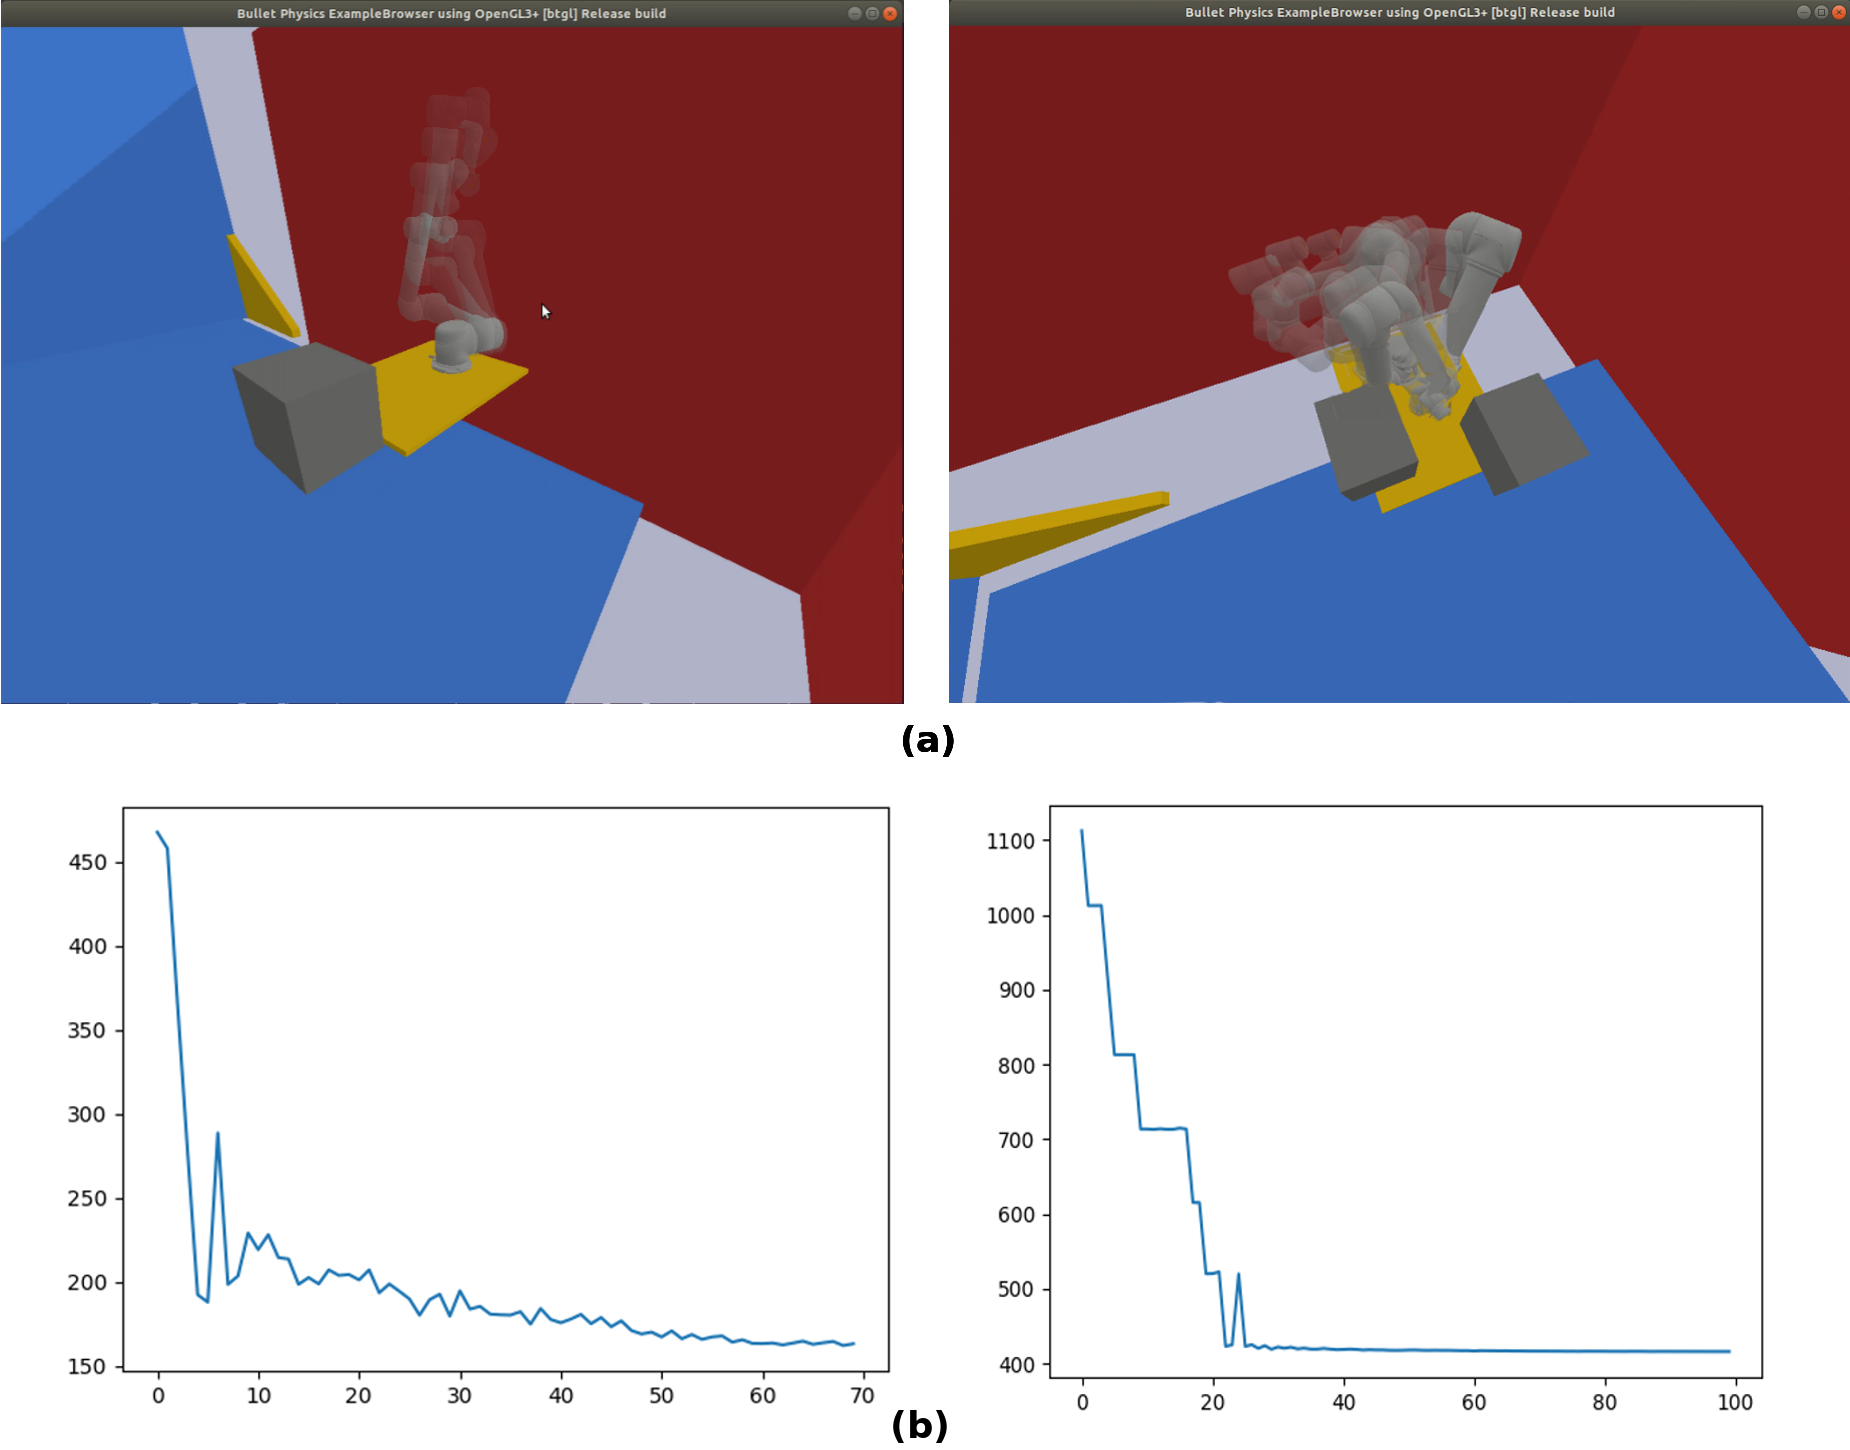
\includegraphics[scale=0.2]{figures/bl-manipulator/joint_trajs.png}
    \caption[Joint-space trajectories using VPSTO]{(a) A few examples of trajectories obtained after joint-space trajectory optimization using VPSTO simulated in PyBullet. (b) The associated cost function plots during the optimization iterations. VPSTO is able to minimize the cost function, which can be denoted from the reducing trend in the cost plots.}
    \label{fig:joint_traj_ur5}
\end{figure}

For the 2-D end-effector space push planning, the simulation results will be shown along with the bi-level optimizer in Section \ref{sec:bl_results}.


\section{Bi-Level Optimization for Non-Prehensile Actions}\label{sec:bi-level-method}

\subsection{Introduction}
 Non-prehensile manipulation has typically received less attention in literature compared to grasp-manipulation. A standard mechanism to robustly push an object from start to goal position while avoiding colliding with objects on the table does not exist. 

A recent work~\cite{iros2022} tackles this problem but assumes contact-rich manipulation in which the target object is attached to the manipulator. This reduces the complexity of the problem by assuming predictable dynamics - the object moves along with the manipulator. Contact-rich manipulator, however, assumes a certain type of gripper that may be not feasible for a given use case.  We concentrate on non-prehensile manipulation in an end-effector agnostic manner that assume the object dynamics to be independent of the end-effector dynamics. The primary challenge in developing a policy to execute such an action is the stochastic outcome on pushing an object: in the absence of priviledged information like friction, weight of the target object, it is impossible to accurately predict the dynamics of the object on a push action. To tackle this, several works have tried to explicitly model the outcome by training a deep neural network on a large amount of push-outcome pairs collected via simulation~\cite{huang2021dipn, huang2021visual, bai2021hierarchical-more}. However, such explicit modeling result in low-generalization making multi-step long-horizon planning of pushing an object from start to goal challenging. 

In recent years, deep reinforcement learning (RL) has shown promising results in various robotics applications. RL algorithms learn to perform a task by maximizing a reward signal, which can be a scalar value that reflects the task's success or failure; or a dense reward indicating the distance from goal. However, RL algorithms have high sample complexity~\cite{rl_sample_complexitiy} and designing the perfect reward function is tricky limiting their application in long-horizon scenarios~\cite{rl_long_horizon} needing complex reward design. 

Moreover, RL algorithms trained for long-horizon tasks are hard to generalize across a wide variety of scene configuration, and out of distribution object shapes and sizes.

In this work, we tackle the problem of object rearrangment using non-prehensile actions by disentangling the space of control and planning. The path planning module generates a feasible trajectory for the robot's end-effector, while the low-level RL controller learns to control the robot's movements to achieve the desired task. In our framework, RL acts as an efficient mechanism for understanding the dynamics of an object on different push actions. Here, the RL controller is trained using a simple objective to push the object quickly to a given goal location. 

In this setting, the low-level controller is unaware of the collision objects and is dependent on a high-level planning module to obtain an optimal collision-free trajectory. At the same time, the high-level planning module predicts the most optimal trajectory for the given RL controller. The framework is trained using bi-level optimization: the high-level planning module is optimized on the cost of execution of the low-level controller. 

A global RL policy solves the task of manipulating an object from start to goal position end-to-end using a single policy. Such a controller simultaneously solves the control task (understanding the dynamics of the system) and the planning task (a collision-free optimal trajectory from start to goal). 
Compared to training a global RL model for non-prehensile object manipulation, our framework, based on a bi-level optimization objective can have several advantages: 

\begin{enumerate}
    \item \textbf{Better task-specific performance:} Non-prehensile object manipulation tasks can be highly varied and complex, and a single global RL model may not be able to handle all tasks equally well. In contrast, a bi-level optimization approach can generate task-specific plans that are optimized for each individual task, resulting in better performance. 
    \item \textbf{Improved sample efficiency:} Non-prehensile object manipulation tasks typically require a large number of samples to train an RL model effectively. A bi-level optimization approach can reduce the number of samples required by using the high-level planning module to generate a task-specific collision-free plan, which can simplify the RL objective to only push to a goal location. 
    \item \textbf{Better interpretability:} A bi-level optimization approach separates the control of the task-specific plan and the low-level actions, making it easier to understand how the system operates and diagnose issues. In contrast, a global RL model can be more opaque and difficult to interpret. 
    \item \textbf{Ability to handle constraints:} Non-prehensile object manipulation tasks often have constraints, such as avoiding collisions or maintaining balance. A bi-level optimization approach can incorporate these constraints into the high-level planning module and use them to guide the low-level actions. 
\end{enumerate}

In contrast, a global RL model may struggle to handle constraints effectively, as designing an appropriate reward can be tricky. 

\subsection{Related Work}

Push-based non-prehensile manipulation can be divided into push-to-grasp, such as pushing objects in clutter to make them graspable~\cite{huang2021dipn, huang2021visual} or sliding an object to the edge of the table~\cite{pregraspsliding, King-2013-7735} and push-to-goal to push an object from a start to a goal position~\cite{iros2022, icra2018, moura2022non, bai2021hierarchical-more}. The latter line of work can further be classified as contact-rich manipulation either by sliding by the top~\cite{xu2021cocoi, song2019object, icra2018, iros2022} or by the side~\cite{moura2022non}. 

We aim to tackle push-to-goal through push-by-striking manipulation. Push-by-striking loses the contact-rich assumption and thus disentangles the dynamics of the object from the manipulator dynamics removing the constraints in the type of end-effector - as the end-effector strikes an object, the outcome of the object state is independent of the end-effector state. 

RL has been applied in various robotics applications, including grasping~\cite{grasp1, grasp2,grasp3}, manipulation~\cite{manipulation1, manipulation2}, and locomotion~\cite{locomotion1, locomotion2}. Recently there has been a lot of work~\cite{residual1, residual2, residual3} on combining RL with classic controllers and primitives to improve their performance. RL-based methods have also shown promising results in performing non-prehensile object manipulation tasks. For instance, Tan et al.\cite{hierarchical-rl} proposed a hierarchical RL method for non-prehensile object manipulation, where the high-level policy generates a sequence of subtasks, and the low-level policy learns to execute each subtask. Zhang et al.\cite{zhang-rl} proposed a hierarchical RL framework that combines the advantages of both model-based and model-free methods for non-prehensile object manipulation.

Path planning algorithms are also widely used in robotics applications, including object manipulation~=\cite{planning1, planning2, planning3}. Path planning algorithms generate a feasible trajectory for the robot to perform the task. Various path-planning algorithms have been proposed, including sampling-based methods\cite{planning1} and optimization-based methods\cite{planning2}. While other path-planning approaches would build a path without taking into account the capabilities of the lower-level controller, our trajectory optimization model samples optimal trajectories by considering the capability of our low-level RL controller. Our neural network is aware of the limitations and capabilities of the lower-level RL controller. 

\subsection{Task Specification}
\label{sec:task-specification}

We consider the task of pushing a target object from an initial pose to a goal pose on a tabletop scene with multiple movable collision objects. The environment consists of a planar surface with dimensions of 0.8m $\times$ 0.8m, upon which up to four movable objects are randomly placed. The target object is a rectangular block with dimensions 0.05m $\times$ 0.05m $\times$ 0.1m, and the robot manipulator is a Franka-Panda arm with two-fingered gripper; however, our framework is independent of the type of gripper and can be extended to any end-effector setting (point contact, area contact, contact-rich, etc.). The manipulator interacts with the environment by pushing the target object, using the tip of the arm as the pushing point. The goal location is specified as the pose of the target object on the given tabletop scene. 

\subsection{Proposed Framework}

Our proposed approach involves two modules: a path planning module and a low-level RL controller. The path planning module generates an optimal collision-free trajectory for the robot's end-effector, while the low-level RL controller controls the robot's movements to accomplish the task objectives. Fig.~\ref{fig:pipeline} illustrates the proposed approach.

\begin{figure}
    \centering 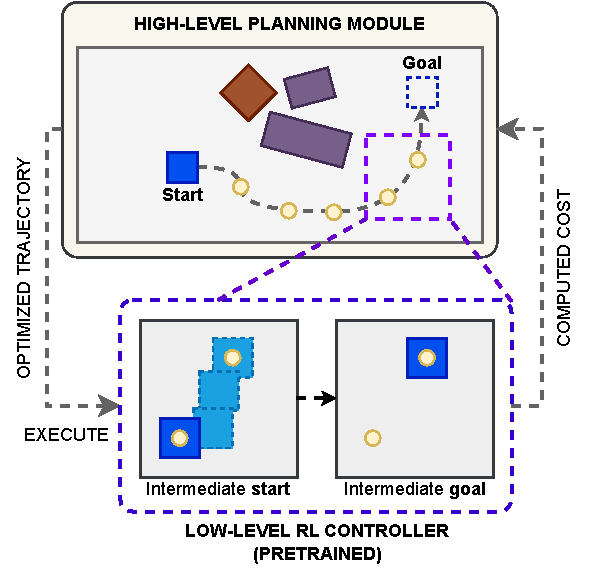
\includegraphics[scale=0.8]{figures/bl-manipulator/pipeline.v9.pdf} 
    \caption[Bi-level optimization pipeline]{Our bi-level optimization framework to solve the task of non-prehensile object manipulation in a cluttered tabletop rearrangement scene. We make use of a low-level RL controller that is trained to reach a short goal. The high-level planning module predicts a set of waypoints that is most optimal for the low-level RL controller to execute. The purple and brown objects indicate obstacles (collision-objects); dark-blue squares indicate the target object and the light-blue squares indicate the trajectory taken by the RL-controller between a set of intermediate waypoints predicted by high-level planning module.}
    \label{fig:pipeline}
\end{figure}

\subsubsection{Low-level RL Controller}
\label{sec:low-level-rl}

Our RL controller learns to simply push a target object from a start to goal location on a tabletop scene. Our controller is trained without any obstacles on the table and is optimized to approach the goal location quickly. Our state space consists of the set of poses taken by the target object, which is being pushed by the RL controller. The action space is defined as a set of 8 discrete equidistant points on the perimeter of the target object and 8 different push angles at each of these 8 points. The objective of the controller is to learn a policy that maximizes the expected cumulative reward, where the reward is the dense negative distance from the current pose to the goal location. The distance metric is the Euclidean distance between the centroid of the target object and the goal location.

Formally, the state space is represented by $S \in \mathbb{R}^{6}$, where each element of the state vector represents the position and orientation of the target object. The action space is represented by $A \in \mathbb{R}^{16}$, where each action is a combination of a point on the object and a push angle. Let $s_t \in S$ and $a_t \in A$ denote the state and action at time step $t$, respectively. The state transition is deterministic, and the next state $s_{t+1}$ is computed as the result of applying the push action to the current state $s_t$.

The reward function is defined as 
\begin{equation}
r(s_t, a_t) = -\gamma ||\; \mathcal{C}(s_t) - \mathcal{G}\; ||_2
\end{equation}
where $\gamma$ is a discount factor, $\mathcal{C}(s_t)$ is the centroid of the target object in the current state, and $\mathcal{G}$ is the goal location. The negative distance metric is used to encourage the controller to minimize the distance to the goal location. The discount factor is used to balance the trade-off between short-term and long-term rewards.

The RL controller learns a policy $\pi(s_t)$ that maps states to actions by maximizing the expected cumulative reward. The optimal policy is obtained by solving the Bellman equation, which is given by:
\begin{equation}
\begin{aligned}
    &Q(s_t, a_t) = r(s_t, a_t) \\
    &+\; \gamma \sum_{s_{t+1}} P(s_{t+1}|s_t,a_t) \max_{a_{t+1}} Q(s_{t+1}, a_{t+1})
\end{aligned}
\end{equation}
where $Q(s_t, a_t)$ is the state-action value function, $P(s_{t+1}|s_t,a_t)$ is the transition probability, and $\max_{a_{t+1}} Q(s_{t+1}, a_{t+1})$ is the maximum expected future reward. The policy is then derived from the optimal value function as:
\begin{equation}
    \pi(s_t) = \arg\max_{a_t} Q(s_t, a_t)
\end{equation}

To learn the optimal policy, we employ a deep Q-learning algorithm that uses a neural network to approximate the value function. The network takes the state as input and outputs the value for each action in the action space. We use the Adam optimizer to minimize the mean squared error between the predicted and target Q-values.

\subsubsection{High-Level Path Planning Module}
\label{sec:path-planning-module}
The high-level planner generates a feasible trajectory for the object being pushed by the manipulator, taking as input the initial and final configurations of the object, and producing a sequence of intermediate via-points that the low-level controller must push it along. In our case, it is important to plan the high-level trajectory for the object instead of the manipulator itself, as is done in case of contact-rich manipulation. This is because, the behavior of the manipulator and the object being pushed are different. Pushing in a contact-impoverished manipulation task, the robot's end-effector only contacts the object briefly to give it a push, and the object continues to move without being directly contacted by the manipulator. Due to this, it is not straightforward to predict the object's trajectory based solely on the manipulator's motion, making it more challenging to plan a trajectory directly for the manipulator. It is noteworthy that planning the high-level trajectory for the object, as opposed to the manipulator, provides a robust and gripper-agnostic algorithm that accounts for the mismatches between the manipulator's motion and the object's movement due to striking.

The predicted via-points are collision-free and ensure that the object can be pushed towards the goal location without encountering any obstacles. For high-level planning, we use the VPSTO algorithm, a stochastic sampling-based optimization method. VPSTO evaluates candidate trajectories by estimating the per-iteration cost function on a simulator running the low-level RL controller, which effectively captures the manipulator and environment dynamics. The cost function incorporates joint cost, collision cost, and boundary cost as explained in the following section.

\subsection{Designing the bi-level optimization objective}

As can be seen in Fig.~\ref{fig:pipeline}, the high-level planning module predicts an optimal trajectory for the end-effector. In other words, the predicted trajectory, $\mathcal{T}$, comprising of a set of via-points, $\mathcal{V}$, is optimal in terms of the manipulator's joint cost, $\mathcal{J}$, as it tries to execute the trajectory. 

To obtain the optimal trajectory for a given scene made of multiple obstacles, VPSTO optimizes the following cost objective, $\mathbb{J}$ computed as:
\begin{equation}
    \mathbb{J}(\pi, \mathcal{V}) = \alpha\mathcal{J} + \beta\mathcal{X} + \gamma\mathcal{B} 
\end{equation}
where $\pi$ is our low-level RL policy as defined in Sec.~\ref{sec:low-level-rl}. $\mathcal{X}$ and $\mathcal{B}$ are the collision and out-of-boundaries cost, respectively. $\alpha$, $\beta$, and $\gamma$ are the scaling parameters to normalize the three different metrics.  $\mathcal{J}$ is calculated based on the first-order change in manipulator's joint angles, while the collision cost, $\mathcal{X}$, reflects the change in obstacle positions in the scene. The out-of-boundary cost, $\mathcal{B}$, is calculated as the frequency of workspace boundary violations. Note that the joint angles are obtained after simulating the manipulator's movement using the low-level RL controller in PyBullet. For each of the via-point $\{v_i\}_{i=1}^{\mathcal{K}-1} \in \mathcal{V}$, the RL controller is executed to push the object from $v_i$ to $v_{i+1}$; here $\mathcal{K}$ is the number of via-points predicted by the planning module. The total joint cost is then computed as:
\begin{equation}
\label{eqn:joint-cost}
    \mathcal{J} = \sum_{i=1}^{\mathcal{K}-1} j(v_i, v_{i+1})
\end{equation}
where $j$ indicates the local cost of moving the target object between the intermediate via-points. Furthermore, our approach mainly focuses on the pushing behavior of the manipulator on the plane of the table; collisions can be assumed to be marked by positional displacements of obstacles according to the task specification in Section~\ref{sec:task-specification}.

\subsection{Simulation Results}\label{sec:bl_results}

We test our bi-level optimizer on a few tabletop scenarios, involving one or more obstacles of varied shapes and sizes in the PyBullet simulator. Figure \ref{fig: bl_qualitative} shows the trajectories predicted by our bi-level approach, while avoiding collisions and minimizing joint cost within the workspace bounds. Figure \ref{fig:bl_sim} indicates the predicted trajectory when run in the PyBullet simulator using our low-level push controller. Additional simulation results on other test cases can be found at: \url{https://www.dropbox.com/sh/mf8j0kq4mv53wct/AABVdITIHCfNBtqHMphnJcSia?dl=0}.


\begin{figure*}
    \centering 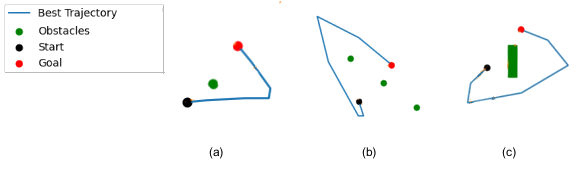
\includegraphics[width=0.8\linewidth]{figures/bl-manipulator/trajectories-v2.png} 
    \caption[Bi-level optimizer trajectories]{Trajectories predicted by our framework. Our framework successfully avoids trajectories and is conservative when choosing a path. Note that the positions shown here are placeholders to indicate the locations of the centres of various objects. (a) shows a trajectory with a simple case of a single collision object, (b) shows a more complicated case when there are multiple collision objects. The obstacle sizes are so big that it is not possible for the manipulator to go between them, so it takes an alternate route around the obstacles. (c) shows a case with an elongated obstacle. Even though the trajectories may not look the most optimal in terms of Euclidean distance, these trajectories are near-optimal with respect to joint and collision cost. }
    \label{fig: bl_qualitative}
\end{figure*}

\begin{figure*}[t!]
    \centering
    \begin{subfigure}[t]{0.5\textwidth}
        \centering
        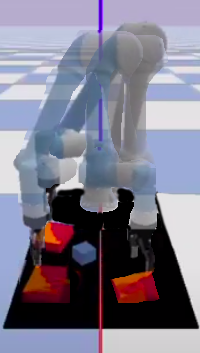
\includegraphics[height=1.8in]{figures/bl-manipulator/bl_sim.png}
    \end{subfigure}%
    ~ 
    \begin{subfigure}[t]{0.5\textwidth}
        \centering
        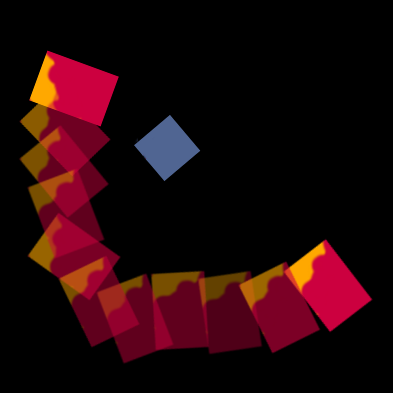
\includegraphics[height=1.8in]{figures/bl-manipulator/2d_object.png}
    \end{subfigure}
    \caption[Bi-level simulation in PyBullet]{(a) Trajectories predicted by our framework simulated in PyBullet with our low-level RL push controller. The blue boxes on the black table indicate collision objects(obstacles), (b) The top-view of the object motion as a result of executing the trajectory.}
    \label{fig:bl_sim}
\end{figure*}

\section{Discussions and Conclusion}

In this chapter, we adapted the Via-point-based Stochastic Trajectory Optimization(VPSTO) trajectory optimizer for manipulator path planning tasks, using PyBullet's mesh overlap technique to detect collisions. We presented a few simulation results obtained from joint-space trajectory planning using VPSTO. We then proposed a framework for disentangling non-prehensile long-horizon manipulation into planning and control. Our approach predicts a collision-free trajectory using VPSTO and simplifies the control component's task by reducing it to moving the object towards the next via-point. In the future, one can reduce the planning time for our offline bi-level optimizer by curating a dataset of start-goal pairs and their optimal trajectories. A neural network can be trained to learn these configuration-to-trajectory mappings, and can be used in real-time during inference to quickly obtain optimal manipulator trajectories. Further, more ablation studies can be performed by replacing the optimizer and the push controller in our bi-level optimization framework. Overall, our proposed framework is a promising step towards achieving more efficient and flexible non-prehensile manipulation.